% -*- LaTeX -*-

% Add proof example to 54
% Resolution: inference rule, proof trees, semantic interpretation,
% rule interpretation, soundness and completeness

\documentclass[handout,x11names,unknownkeysallowed]{beamer}
%\documentclass[x11names]{beamer}
\usepackage{beamerthemeUAB}
\usepackage{verbatim}
\usepackage{color}
\usepackage{multirow}
\usepackage{cite}
%\usepackage{amsthm}
%\setbeamertemplate{theorems}[numbered]
%\newtheorem{proposition}{Proposition}
%\newtheorem{cor}{Corollary}
% -*- LaTeX -*-

\usepackage{subfigure,bm}
\usepackage{multicol}
\usepackage{amsmath}
\usepackage{epsfig}
\usepackage{graphicx}
\usepackage[all,knot]{xy}
\usepackage{marvosym}
\xyoption{arc}
\usepackage{url}
\usepackage{multimedia}
\usepackage{hyperref}
\usepackage[english]{babel}
\usepackage[latin1]{inputenc}
\usepackage{times}
\usepackage{caption}
%\usepackage[T1]{fontenc}
% Or whatever. Note that the encoding and the font should match. If T1
% does not look nice, try deleting the line with the fontenc.
\newcommand{\conv}{\stackrel{\mathbb{D}}{\longrightarrow}}
\newcommand{\cons}{\stackrel{p}{\longrightarrow}}
\newcommand{\nc}{\newpage \clearpage}
\newcommand{\etal}{\textit{et al.}}

\def\boldp{\mathbf p}
\def\btheta{\bm \theta}
\def\bpi{\bm \pi}

\title[] % (Called "`Short Title"', optional, use only with long paper titles)
{Matrix Review}

%\subtitle{EPID 753} % (optional)

\author[Dustin Long, PhD] % (optional, use only with lots of authors)
{Dustin~Long, PhD}


\institute[UAB]
{
  Department of Biostatistics\\
	University of Alabama at Birmingham

}

\def\insertcopyright{$\copyright$ 2019 by Dustin Long}
\def\insertslideinfo{\insertshorttitle}

\subject{}
% This is only inserted into the PDF information catalog. Can be left
% out. 



% This code is not needed since the logo is on every page in the lower left-hand corner
%\pgfdeclareimage[height=0.5cm]{university-logo}{unc-gillings-school-of-public-health-logo.png}
%\logo{\pgfuseimage{university-logo}}


% Delete this, if you do not want the table of contents to pop up at
% the beginning of each subsection:
%\AtBeginSubsection[]
%{
%   \begin{frame}<beamer>
%     \frametitle{Outline}
%     \tableofcontents[currentsection,currentsubsection]
%   \end{frame}
% }


% If you wish to uncover everything in a step-wise fashion, uncomment
% the following command: 

%\beamerdefaultoverlayspecification{<+->}

%\input macros.tex

\date[Matrix Review]{August 29, 2019}

\newcommand{\beamitem}{\begin{itemize}[<+-|alert@+>]}
%\newcommand{\beamitem}{\begin{itemize}}
%\newcommand{\etal}{\textit{et al.}}

%%%%%%%%%%%%%%%%%%%%%%%%%%%%%%%%%%%%%%%%%%%%%%%%%%%%%%%%%%%%%%%%%%%%%%
\begin{document}

\begin{frame}
  \titlepage
\end{frame}

\begin{frame}
Outline:
\begin{itemize}
\item Matrix Review
\end{itemize}

\end{frame}



%%%%%%%%%%%%%%%%%%%%%%%%%%%%%%%%%%%%%%%%%%%%%%%%%%%%%%%%%%%%%%%%%%%%%%

\begin{frame}
Matrix review
\begin{itemize}
\item $\bm{A}_{r \times c} = \left[ \begin{array}{cccc}
													a_{11} & a_{12} & \ldots & a_{1c}\\
													a_{21} & a_{22} & \ldots & a_{2c}\\
													\vdots & \vdots & \vdots & \vdots \\
													a_{r1} & a_{r2} & \ldots & a_{rc}\\ 
													\end{array}\right]$
													
\item Vectors (one column) and scalars (one row and one column) are special types of matrix.
\end{itemize}
\end{frame}





\begin{frame}
Matrix review
\begin{itemize}
\item Square matrices (r=c) and diagonal matrices (only elements are $a_{ij}$ where $i=j$ and 0 elsewhere)
\item Symmetric matrix has $a_{ij} = a_{ji}$ for all $i, j$
\end{itemize}
\end{frame}

\begin{frame}
Matrix review
\begin{itemize}
\item Trace of a matrix trace$(\bm{A}) = \sum_{i=1}^c a_{ii}$, sum of diagonals
\item Transpose of $\bm{A}$: $\bm{A}_{r \times c}'$ flip matrix on diagonal
\item $\bm{A}_{r \times c} + \bm{B}_{r \times c} = \{a_{ij} + b_{ij}\}_{r \times c}$
\item Five types of multiplication: elementwise, matrix, scalar, Kronecker, horizontal direct product 
\item Most common is matrix multiplication which must have conformable dimenstions
\item $\bm{A}_{r \times c} \ast \bm{B}_{r \times c}$ does not work (non-conformable)
\item $\bm{A}_{r \times c} \ast \bm{B}_{c \times r}$ does (conformable)
\item $	\left[ \begin{array}{cc} 1 & 2 \\ 1 & 3 \\ 1 & 5 \\ \end{array}\right] \ast 
				\left[ \begin{array}{ccc} 1 & 2 & 2\\ 1 & 3 & 4 \\ \end{array}\right] 
			= \left[ \begin{array}{ccc} 3 & 8 & 10 \\ 4 & 11 & 14 \\  6 & 17 & 22 \\ \end{array}\right]$

\end{itemize}
\end{frame}


\begin{frame}
Matrix review
\begin{itemize}
\item Commutative law works for addition
\item Distributive laws:  Remember that $\bm{A} \ast \bm{B} \neq \bm{B} \ast \bm{A} $ except in special cases
\item $(\bm{A} \ast \bm{B})' = \bm{B}' \ast \bm{A}'$
\item Determinant: $|\bm{A}|$, only for square matrices
\item $	\left| \begin{array}{cc} a & b \\ c & d \\ \end{array}\right| = ad-bd$
\end{itemize}
\end{frame}

\begin{frame}
Matrix review
\begin{itemize}
\item Determinant is a index of the variability in a matrix
\item Larger magnitude implies larger variability
\item Determinant visualization \\
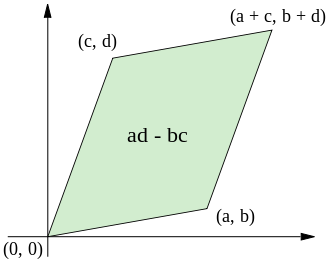
\includegraphics[width=0.5\textwidth]{determinant.png}
\end{itemize}
\end{frame}


\begin{frame}
Matrix review
\begin{itemize}
\item Rank, the number of linearly independent columns in a matrix (typically the number of columns)
\item A less than full rank matrix, where rank is less than number of columns, is called singular
\item A full rank matrix is called nonsingular
\item The inverse of a matrix, $\bm{A}^{-1}$, exists for all nonsingular square matrices such that $\bm{A} \ast \bm{A}^{-1} = \bm{I}$
\item For singular square matrices, the generalized inverse $(\bm{A}^{+})$ exists but is not unique
\item Eigenvalues, any number $\lambda$ that is the solution to the equation $|\bm{A}-\lambda\bm{I}|$
\end{itemize}
\end{frame}

\begin{frame}
Matrix Review: Statistical quantities
\begin{itemize}
\item Sum of Squares
\item The matrix $\bm{A}*\bm{A}'$ has elements $\sum a_{ij}*a_{rs}$ with diagonal elements  $\sum a_{ij}^2$
\item Covariance matrix
\item $\bm{S} = \bm{D'D}\frac{1}{N-1}$ where $\bm{D}_{r \times c}$ is $\bm{A}_{r \times c}$ subtracting the column mean from each corresponding column entree
\item OR $\bm{D}_{r \times c} = (\bm{I}_{r \times r} - \frac{1}{c}\bm{1}_{r \times r})\bm{A}_{r \times c}$
\end{itemize}
\end{frame}


\begin{frame}
Matrix Review
\begin{itemize}
\item Can use matrices to represent a series of linear equations, e.g.

\begin{eqnarray*}
5x + 7y & = & -11\\
8x + 4y & = & 4 \\
5x+5y & = & -5 
\end{eqnarray*}
													
\item $\bm{A}_{2 \times 2} = \left[ \begin{array}{cc}
													5 & 7 \\
													8 & 4 \\
													5 & 5 \\ 
													\end{array}\right]$, 
			$\bm{b}_{2 \times 1} = \left[ \begin{array}{c}
													x  \\
													y  \\
													\end{array}\right]$, 
			$\bm{c}_{2 \times 1} = \left[ \begin{array}{c}
													-11  \\
													4  \\
													-5  \\ 
													\end{array}\right]$.
\item Thus, the series of equations can be written as
\begin{equation*}
\bm{A} * \bm{b} = \bm{c}
\end{equation*}
\end{itemize}
\end{frame}

\begin{frame}
\begin{center}
Questions?
\end{center}

\end{frame}



\end{document}